\chapter{Fundamentação Teórica}\label{cap:fundamentacao-teorica}

Em desenvolvimento. Fundamentação Teórica para os principais pontos da
na pesquisa:

\begin{itemize}
\item Superpixel
\item Geração de Redes Complexas
\item Matriz de Co-ocorrência
\item \gls{LCU}
\item Aprendizado Semi-supervisionado
\item Processamento de imagem
\end{itemize}



\section{Aprendizado Semi-supervisionado vs. Transdução}\label{sec:teorica-aprendizado-semi-supervisionado}

Existem três principais categorias de aprendizado de máquina:
aprendizado supervisionado, aprendizado não-supervisionado e
aprendizado semi-supervisionado. No aprendizado supervisionado durante
a etapa de treinamento existe uma base de dados totalmente rotulada,
no aprendizado não-supervisionado não é disponibilizado nenhum
rotulamento dos dados. Enquanto isso, o aprendizado
semi-supervisionado está entre essas duas categorias.

O aprendizado semi-supervisionado é um método de aprendizado de máquina
que envolve o uso de um grande volume de dados não rotulados e um
pequeno volume de dados rotulados para treinar modelos de aprendizado
de máquina.

Formalmente, pode-se definir o aprendizado semi-supervisionado da seguinte maneira:

\begin{quote}
Dado um conjunto de dados de treinamento $ X = \{x_1, x_2, \ldots, x_n\} $
onde apenas um subconjunto  $ Y = \{y_1, y_2, \ldots , y_m\} $ tal que $ (m < n) $ tem rótulos
correspondentes, o objetivo do aprendizado semi-supervisionado é usar
tanto o conjunto de dados rotulado quanto o não rotulado para aprender
a função $ f: X \rightarrow Y $ que pode prever o rótulo $ y $ para um novo
exemplo $ x $.
\end{quote}

O aprendizado semi-supervisionado é baseado na suposição de que os
dados não rotulados podem fornecer informações adicionais que podem
ser usadas para melhorar a precisão do modelo de aprendizado de
máquina. Isso é feito através de várias técnicas, como a propagação de
rótulos, onde os rótulos são propagados dos dados rotulados para os
dados não rotulados, ou a aprendizagem auto-supervisionada, onde o
modelo é treinado para prever partes dos dados a partir de outras
partes.

Por outro lado, existe um diferente tipo de aprendizado
semi-supervisionado que não realiza a etapa de estimar a função $ f
$. Algoritmos que estimam essa função são descritos como indutivos,
pois após o treinamento, para classificar novos dados, realizam uma
inferência por indução ao aplicar a função estimada.

Em contraponto, existem algoritmos que não estimam tal função e apenas
realizam a inferência direta entre os dados rotulados disponíveis e os
não rotulados. Isso é chamado de transdução e um algoritmo bem
conhecido com essa característica é o classificador K-NN.\@ Na
figura~\ref{fig:induction-vs-transduction} a seguir, é ilustrado as
diferenças entre transdução e indução no processo de aprendizagem:


\begin{figure}[h!]
        \captionsetup{width=12cm}
		\Caption{\label{fig:induction-vs-transduction}
          No aprendizado transdutivo, a inferência em novos exemplos
          ocorre de maneira direta.
        }
		\centering
		\UFCfig{}{\fbox{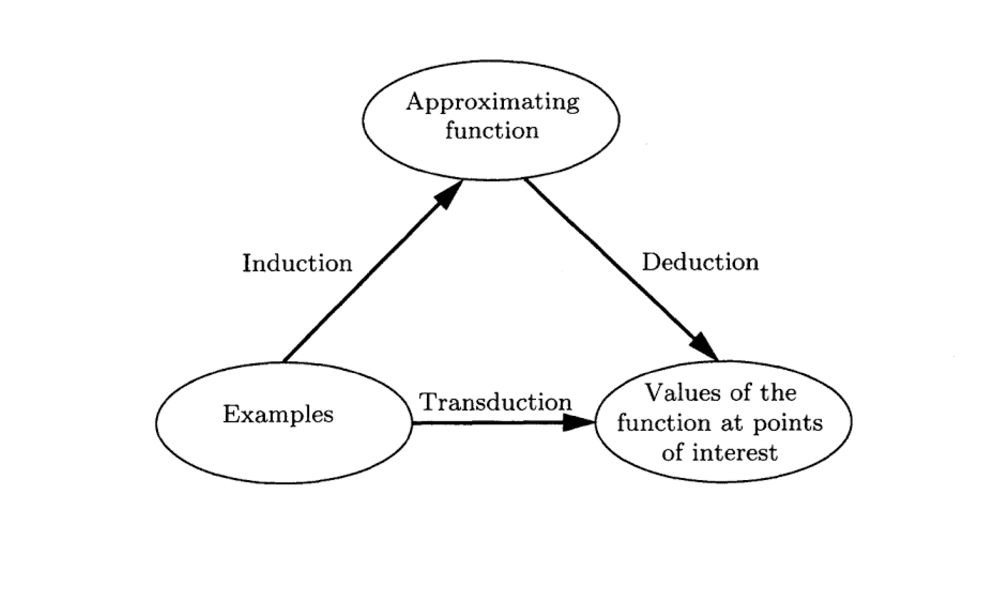
\includegraphics[width=12cm]{figuras/induction_vs_transduction}}}{\Fonte{\cite{vapnik1995}}}
\end{figure}


No texto~\cite{vapnik2006semi}, o criador do famoso algoritmo SVM,
estabelece uma profunda formalização dos problemas de aprendizado
semi-supervisionado e inferência transdutiva. No final do texto, ele declara
algumas reflexões sobre a solução de problemas em aprendizagem de máquina:


\begin{displayquote}

  Solving a problem of interest, do not solve a more general (and therefore worse-
  posed) problem as an intermediate step. Try to get the answer that you really need
  but not a more general one.

  Do not estimate a function if you need to estimate values at given
  points. (Try to perform transduction, not induction.)

\end{displayquote}

Em tradução-livre: \blockquote{Não estime uma função se você precisa estimar
os valores em dados pontos. (Tente executar transdução, não
indução)}. Esse embasamento, é um dos pontos centrais que reforça a motivação deste trabalho.


\section{Aprendizado Ativo}\label{sec:teorica-aprendizado-ativo}

Aprendizado ativo é uma abordagem especializada de aprendizado de
máquina onde o algoritmo pode interagir com o ambiente para obter
melhores informações ou dados de treinamento. Em vez de passivamente
receber todos os dados de treinamento e aprender a partir deles, o
algoritmo de aprendizado ativo tem a capacidade de escolher os dados
dos quais deseja aprender.

Isso é especialmente útil quando os dados de treinamento são caros
para obter ou rotular. O algoritmo pode escolher os exemplos mais
informativos para aprender, economizando recursos.

Formalmente, o aprendizado ativo é um tipo de aprendizado
semi-supervisionado, onde o algoritmo tem acesso a um conjunto de
dados rotulados e não rotulados. O algoritmo seleciona ativamente
exemplos do conjunto de dados não rotulados para serem rotulados e
adicionados ao conjunto de treinamento.

O objetivo do aprendizado ativo é minimizar o erro de generalização,
ou seja, o erro que o modelo fará em novos dados não vistos, com o
mínimo de consultas de rotulagem possível.

\section{Superpixel}\label{sec:teorica-superpixel}

Superpixels é um algoritmo de clusterização em processamento de
imagens que ganhou popularidade nos últimos anos na comunidade de
visão computacional~\cite{SuperpixelSurvey2020}. Em vez de processar
uma imagem pixel por pixel, agrupa-se pixels vizinhos semelhantes em
uma entidade maior, conhecida como superpixel.

O conceito de superpixels foi introduzido para superar as limitações
do processamento pixel a pixel, que não leva em consideração a
estrutura global da imagem. Os superpixels, por outro lado, mantêm a
estrutura da imagem e reduzem a complexidade do processamento de
imagens, tornando-o mais eficiente.

Os superpixels são formados com base na similaridade dos pixels em
termos de cor, intensidade e localização na imagem. Eles são usados em
uma variedade de aplicações, incluindo segmentação de imagem,
rastreamento de objetos, reconhecimento de objetos, entre outros.

Em resumo, os superpixels são uma técnica eficaz para simplificar a
representação de uma imagem e aumentar a eficiência do processamento
de imagens, mantendo a informação visual importante.

Atualmente, já é possível encontrar muitas técnicas baseado em
superpixels com diferentes características, complexidade
computacionais, eficiência e método. No
artigo~\cite{SuperPixelBenchmark2017}, é realizado um benchmark com 15
algoritmos superpixels categorizados em três grupos: basedo em grafos,
baseado em otimização de gradiente e baseado em análise de textura.

\subsection{SLIC}\label{sec:teorica-superpixel-slic}


O algoritmo SLIC (Simple Linear Iterative Clustering) é um método para
a segmentação de imagens baseado em superpixel, é um dos mais simples
e pode ser visto como uma variação do algoritmo k-means expandindo o
espaço euclidiano ao incluir também o espaço de cores. Ele divide uma
imagem em segmentos menores, chamados superpixels, que compartilham
características semelhantes, como cor e textura.

Uma explicação simplificada de como o SLIC funciona pode ser entendida
dessa maneira.:

\begin{enumerate}

\item Inicialização: O algoritmo começa selecionando alguns pixels na
imagem como centros de superpixels. Esses centros são espaçados
uniformemente pela imagem.

\item Atribuição: Em seguida, para cada pixel na imagem, o algoritmo
calcula a distância entre esse pixel e todos os centros de
superpixels. A distância é calculada com base na cor (ou intensidade
de cinza para imagens em preto e branco) e na proximidade espacial. O
pixel é então atribuído ao superpixel cujo centro está mais próximo.

\item Atualização: Depois que todos os pixels foram atribuídos a um
superpixel, o algoritmo recalcula os centros de superpixels como a
média de todos os pixels dentro de cada superpixel.

\item O processo de atribuição e atualização é repetido várias vezes
até que o algoritmo alcance a condição de convergência, ou seja, até
que os centros de superpixels parem de mudar significativamente.

\item O resultado final é uma segmentação da imagem em superpixels, onde
cada superpixel é um grupo de pixels com características semelhantes.

Uma execução do SLIC é possível de ser visualizada a seguir:

\begin{figure}[h!]
        \captionsetup{width=12cm}
		\Caption{\label{fig:slic}
          Execução do algoritmo SLIC na fotografia de um gato.
        }
		\centering
		\UFCfig{}{\fbox{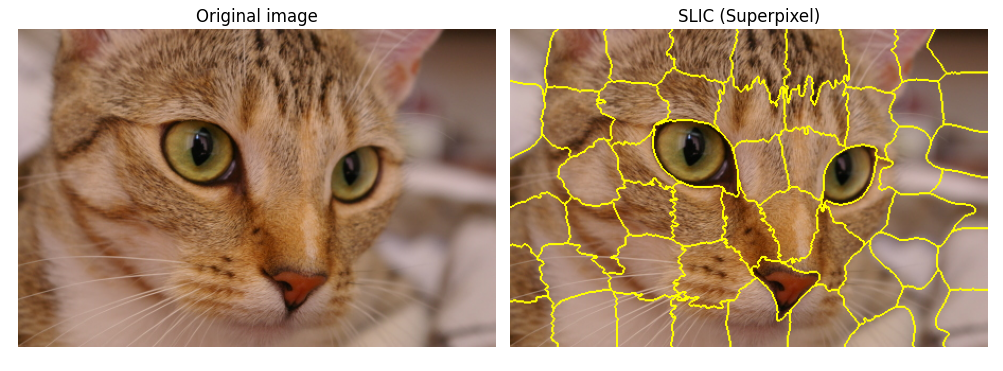
\includegraphics[width=12cm]{figuras/slic}}}{\Fonte{(MANOEL
            VILELA, 2023)}}
\end{figure}


\end{enumerate}

\section{Geração de Redes Complexas}\label{sec:teorica-redes-complexas}

Redes complexas são grafos de alta complexidade. Existem variados
algoritmos para geração de redes complexas
~\cite{ComplexNetworksSurvey2007}. Redes complexas podem ser usadas
como um domínio de dados para realizar tarefas como classificação de
imagens~\cite{ComplexNetworksImageClassification2015}, segmentação de
imagens, identificação de comunidades e também extração de
características~\cite{JarbasComplexNetworks2020}.

Neste trabalho, o uso de redes complexas é realizado de uma maneira
acoplada ao algoritmo de clusterização inicial da imagem (superpixel). Nesse
cenário, cada superpixel gerado na imagem é um vértice e as arestas
são gerados baseado na vizinhança.

Apesar de considerar o tema como redes complexas, esse cenário em
particular gera um grafo planar pela maneira como as arestas são
criadas. Por outro lado, seria possível também modificar a geração da
rede complexa para considerar as arestas do grafo baseado num raio
parametrizado de superpixel em relação a um \textit{treshrold} e
selecionar as k-nn similares como arestas válidas.

Essa etapa de geração da rede complexa é crucial para a execução da
dinâmica coletiva explorada na seção~\ref{sec:teorica-lcu}. Um dos
pontos centrais desse trabalho. Na figura~\ref{fig:complex-networks},
um exemplo de geração de rede complexa é apresentado conectado com a
ilustração~\ref{fig:slic}, ao executar o algoritmo SLIC.\@

\begin{figure}[t]
        \captionsetup{width=12cm}
		\Caption{\label{fig:complex-networks}
          Geração de rede complexa baseado nos superpixels.
        }
		\centering
		\UFCfig{}{\fbox{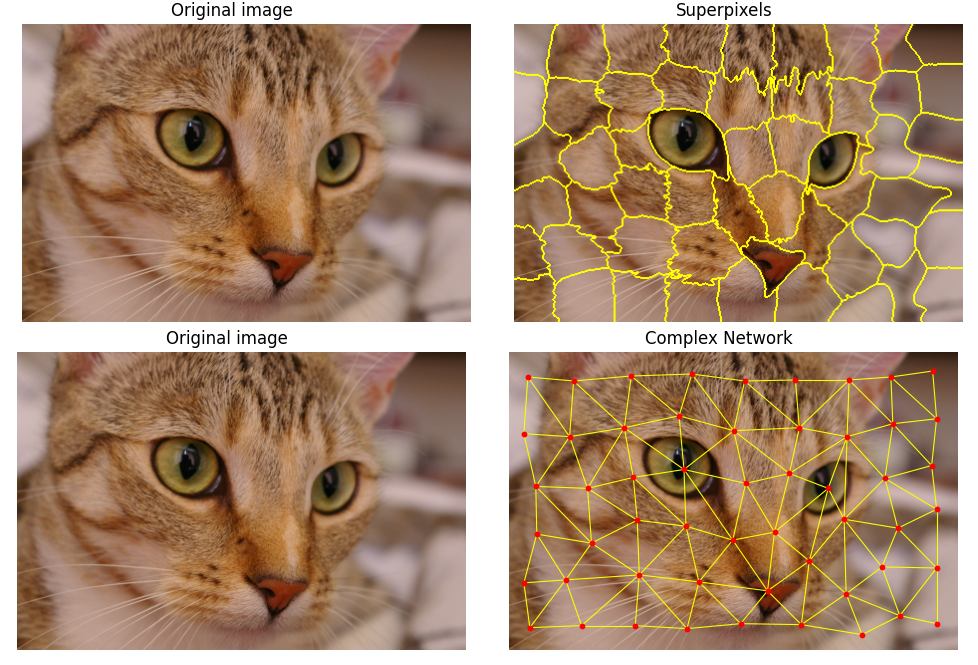
\includegraphics[width=12cm]{figuras/complex-networks}}}{\Fonte{(MANOEL
            VILELA, 2023)}}
\end{figure}
\FloatBarrier{}

\section{Matriz de co-ocorrências}\label{sec:teorica-matriz-co-ocorrencia}

O método de extração de características da matriz de co-ocorrências é
uma técnica utilizada em processamento de imagem e visão computacional
para extrair características texturais de uma imagem~\cite{matrizcoocorrencia2017}.

Formalmente, uma matriz de co-ocorrência C é definida sobre uma imagem
I, para um deslocamento $\Delta x, \Delta y$, como:

\begin{equation}
C_{\Delta x, \Delta y}(i,j)=\sum_{x=1}^n\sum_{y=1}^m\begin{cases} 1, & \text{if }I(x,
                                                       y)=i\text{ e
                                                       }I(x+\Delta x, y+\Delta
                                                       y)=j \\ 0, &
                                                                    \text{caso contrário}\end{cases}
\end{equation}

$C_{\Delta x, \Delta y}(i,j)$ é o número de vezes que o par de pixels com
intensidades i e j ocorre em dois pixels separados pelas distâncias
(horizontal e vertical) na imagem I.

A matriz de co-ocorrência é tipicamente normalizada dividindo cada
elemento pelo número total de pares de pixels na imagem, resultando em
uma matriz de probabilidade de co-ocorrência.

A partir desta matriz, várias características texturais podem ser
extraídas, como contraste, correlação, energia e homogeneidade. Estas
características podem ser usadas para tarefas como classificação de
textura, segmentação de imagem, entre outros.


\section{Métricas de Similaridade}\label{sec:teorica-metricas-de-similaridade}

A ser escrito: distância euclidiana, distância manhattan, distância
jaccard (?), métrica de similaridade exponencial $\exp(\dfrac{-d}{s})$

\section{Métricas de Avaliação}

Existem três métricas que são comumente utilizadas em segmentação
semântica de imagens:

\begin{enumerate}
\item IoU
\item Dice Score (F1)
\item Pixel Accuracy
\end{enumerate}

IoU~\cite{rezatofighi2019generalized}, que significa
\textit{Intersection over Union}, é uma métrica popularmente usada
para medir a precisão de um objeto de segmentação em tarefas de visão
computacional, como detecção de objetos e segmentação semântica.

A métrica IoU calcula a proporção da área de interseção entre a região
estimada e a região real (ground truth) pela área da união dessas duas
regiões. A fórmula para calcular o IoU é:

\begin{equation}
  IoU = \dfrac{\left| A \cap B \right|}{\left| A \cup B \right|}
\end{equation}


Nessa equação, A e B são matrizes de rótulos da imagem onde serão
comparados, por exemplo o A sendo os rótulos estimados e B os reais. O
valor de IoU varia de 0 a 1, onde 1 indica uma correspondência
perfeita entre as caixas delimitadoras previstas e reais, e 0 indica
que não há sobreposição. Em geral, um IoU maior indica uma melhor
precisão do modelo de segmentação.

A métrica mIoU é uma versão para segmentação multi-classe realizando
uma média dos IoU calculando individualmente pra cada classe,
considerando a classe negativa qualquer uma que não seja a classe alvo.

\section{LCU}\label{sec:teorica-lcu}

O algoritmo \gls{LCU} foi desenvolvido por um
brasileiro~\cite{VerriNetworkUnfoldingMap2018}, é uma dinâmica
coletiva baseado em propagação de rótulos numa rede complexa. Essa
dinâmica coletiva é modelada como um sistema dinâmico com geração de
partículas de rotulação nas suas fontes (os vértices rotulados).

Esse algoritmo possuem critérios de sobrevivência das particulas
inspirado em comportamentos da natureza e sociedade. Por exemplo, o
hiperparâmetro $ \lambda $ do algoritmo denota um fator entre 0 e 1 de
competitividade entre as partículas, tornando a sobrevivência delas
mais difícil ao percorrer o grafo. Embora as partículas nasçam nos
vértices, a competição por dominação acontece nas arestas. No final, o
vértice será marcado com o novo rótulo baseado no tipo de partícula
que mais conseguiu dominar arestas desse vértice.

Nesse caso particular, a implementação proposta é ligeiramente
diferente da proposta originalmente, pois a rede complexa no cenário
que o autor propõe as arestas não possuem peso. A modificação é
realizada para incluir a similaridade de imagem entre dois
superpixels, dessa maneira é criado um fator de aumento da
probabilidade das partículas visitarem os nós mais promissores. Como
discutido na seção
~\ref{sec:teorica-aprendizado-semi-supervisionado}, esse cenário de
aprendizado é semi-supervisionado transdutivo: poucos rótulos estão
disponíveis e nenhuma função de inferência é estimada. A inferência
acontece diretamente entre os pontos rótulados e os não-rotulados.


\begin{figure}[!h]
        \captionsetup{width=12cm}
		\Caption{\label{fig:lcu-partial}
          Rede complexa preparada com anotação parcial para execução do \gls{LCU}
        }
		\centering
		\UFCfig{}{\fbox{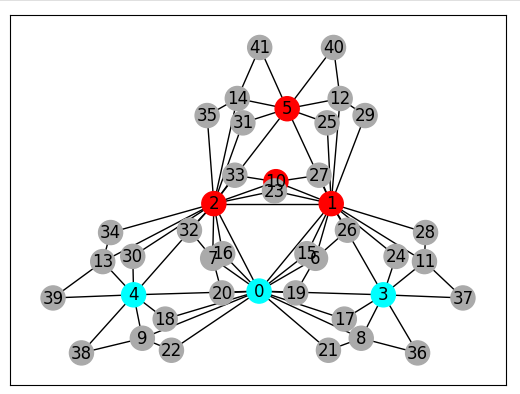
\includegraphics[width=12cm]{figuras/lcu-partial}}}{\Fonte{(MANOEL
            VILELA, 2023)}}
\end{figure}
\FloatBarrier{}

\begin{figure}[!h]
        \captionsetup{width=12cm}
		\Caption{\label{fig:lcu-done}
          Execução do \gls{LCU} finalizada.
        }
		\centering
		\UFCfig{}{\fbox{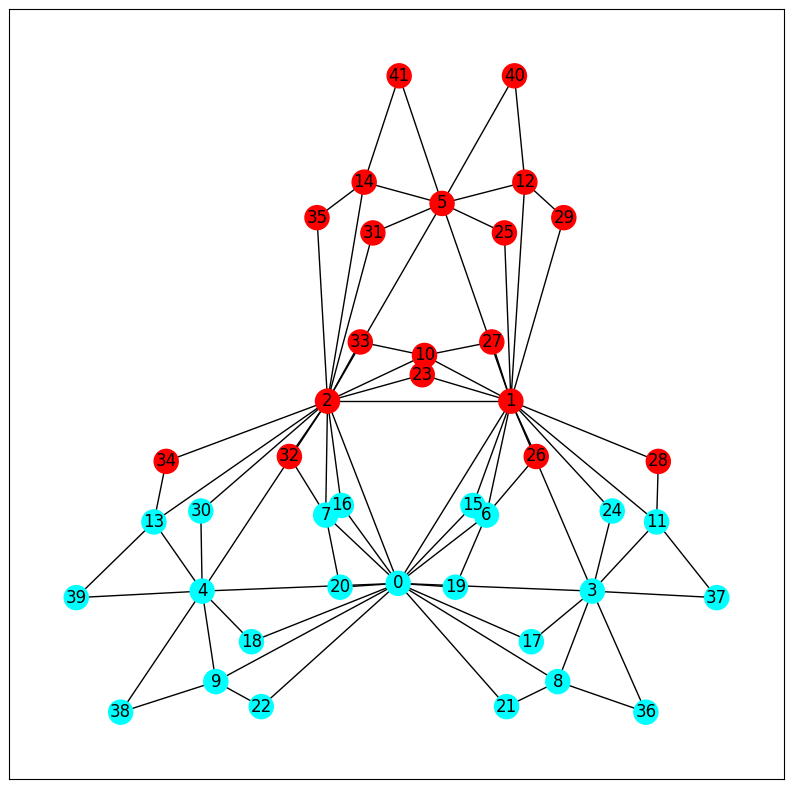
\includegraphics[width=12cm]{figuras/lcu-done}}}{\Fonte{(MANOEL
            VILELA, 2023)}}
\end{figure}
\FloatBarrier{}

Nas figuras~\ref{fig:lcu-partially-annotated} e~\ref{fig:lcu-done} é
possível ver a execução do algoritmo numa rede complexa densa
aleatória, no final da execução os rótulos são propagados
semanticamente baseado na disputa entre as partículas.


\section{EGSIS}\label{sec:teorica-egsis}

A ser escrito, algoritmo agregador que une todas as partes.
